\documentclass[12pt,a4paper]{article}

\usepackage[T2A]{fontenc} %поддержка кириллицы
\usepackage[utf8]{inputenc} %кодировка текста: koi8-r или utf8 в UNIX, cp1251 в Windows
\usepackage[english,russian]{babel} 
\usepackage[left=2cm,right=1.5cm,top=2cm,bottom=2cm]{geometry} 
\usepackage{tabularx} 
\usepackage{graphicx} 
\usepackage{amsmath} %отображение математической нотации
\usepackage{float}
\usepackage{caption, subcaption} %подписи
%\usepackage{array}
%\usepackage{amsmath,booktabs}
%\usepackage{tabu}
\usepackage{indentfirst}%отступ вначале параграфа
%\usepackage{pscyr} %???
%\usepackage{natbib}
%\usepackage{ragged2e} %для таблиц
 
\captionsetup[table]{labelsep = endash, singlelinecheck=false}
\captionsetup[figure]{name = Рисунок, labelformat=simple, labelsep = endash}

\begin{document}

\include{title}

\paragraph{Цель работы:}Ознакомление с экспериментальными методами построения областей устойчивости линейных динамических систем и изучение влияния на устойчивость системы её параметров.%*-без нумерации
\paragraph{Вариант задания.} $T_1$ = 2.25
\newpage
\begin{center}
    \section{Построение границы устойчивости на плоскости двух параметров $K$ и $T_2$ методом математического моделирования}
\end{center}
\par
На рисунке 1 представлена схема моделирования для системы с заданными параметрами.
\begin{figure}[h!]
	\centering
	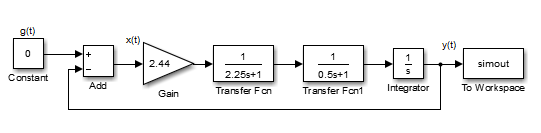
\includegraphics[width=0.9\linewidth]{scheme.png}
	\caption{Структурная схема моделируемой системы}
\end{figure}
 
Будем менять значение $T_2$ и подбирать коэффициент передачи $K$ таким образом, чтобы система находилась на границе устойчивости. Данные, необходимые для построения границы устойчивости приведены в таблице 1.
\begin{table}[h!]
	\caption{Данные, необходимые для построения границы устойчивости системы}
	\renewcommand{\arraystretch}{1.8} %строки
	%\renewcommand{\tabcolsep}{1cm} %столбцы
	\begin{tabular}{|c|c|c|c|c|c|c|c|c|c|c|}
		\hline $T_2$ & 0,1 & 0,5 & 1 & 1,5 & 2 & 2,5 & 3 & 3,5 & 4 & 5 \\
		\hline $K$ & 10,44 & 2,44 & 1,45 & 1,1 & 0,94 & 0,84 & 0,78 & 0,73 & 0,69 & 0,66 \\
		\hline
	\end{tabular}	
\end{table} 
Графики переходных процессов для устойчивой системы, неустойчивой и системы, находящейся на границе устойчивости представлены соответственно на 2, 3 и 4 рисунках.
\begin{figure}[H]
	\centering
	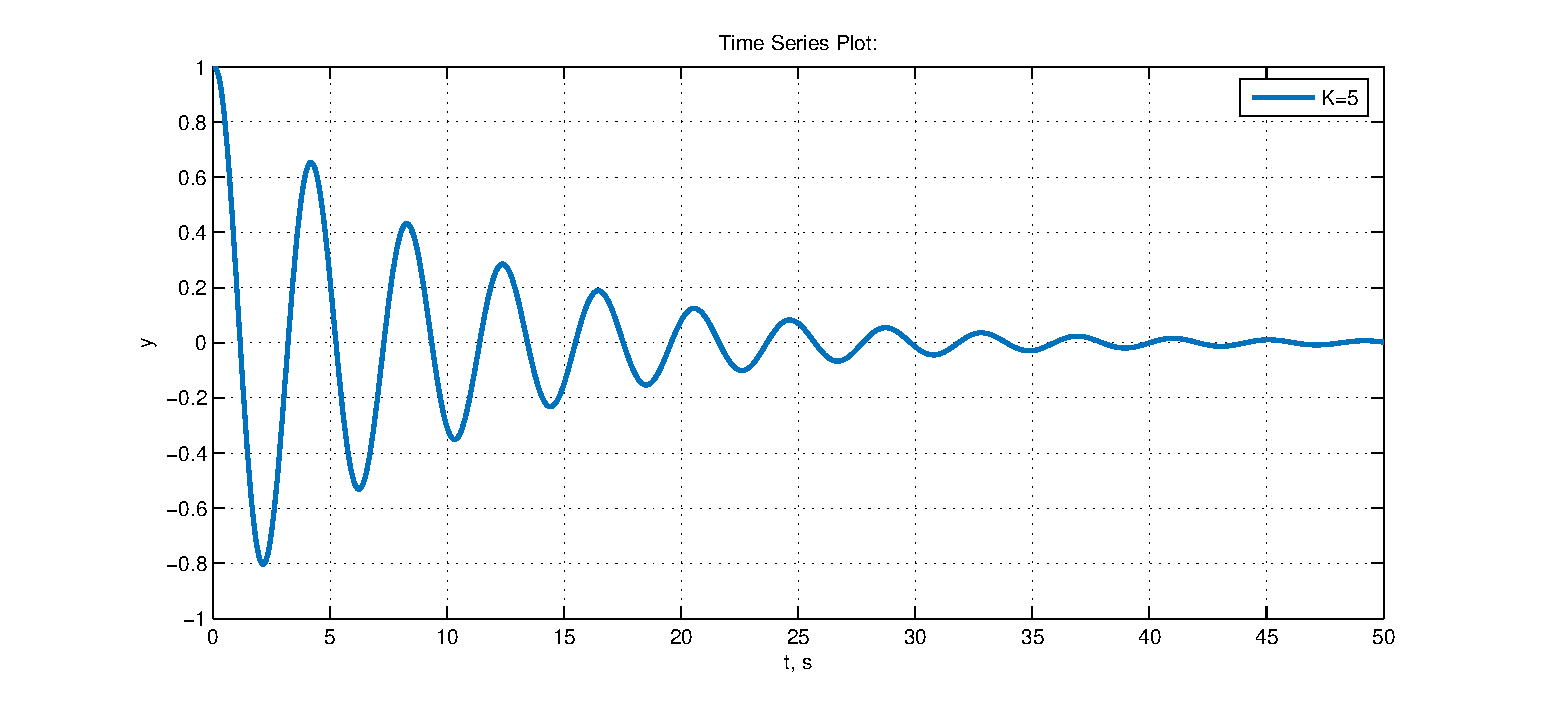
\includegraphics[width=1\linewidth]{second.eps}
	\caption{Система устойчива}
\end{figure}
\begin{figure}[H]
	\centering
	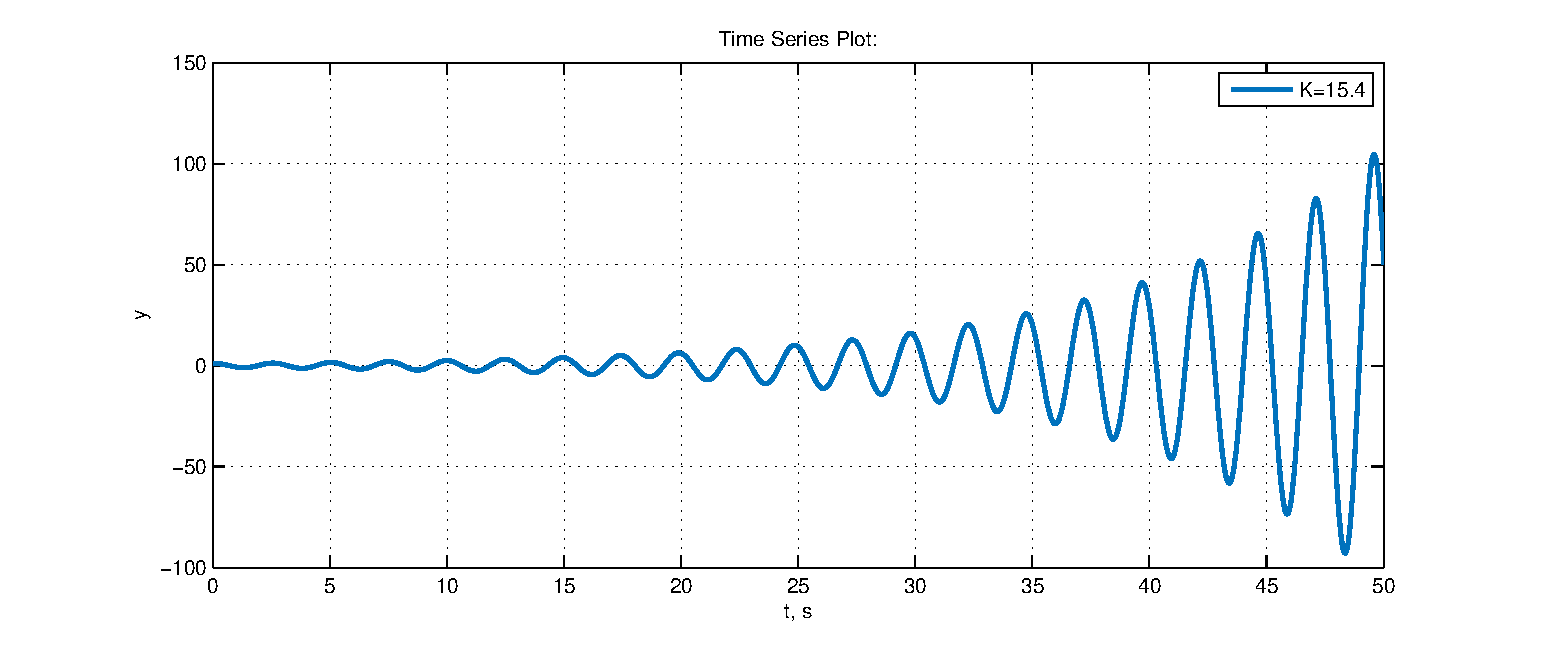
\includegraphics[width=1\linewidth]{third.eps}
	\caption{Неустойчивая система}
\end{figure}
\begin{figure}[H]
	\centering
	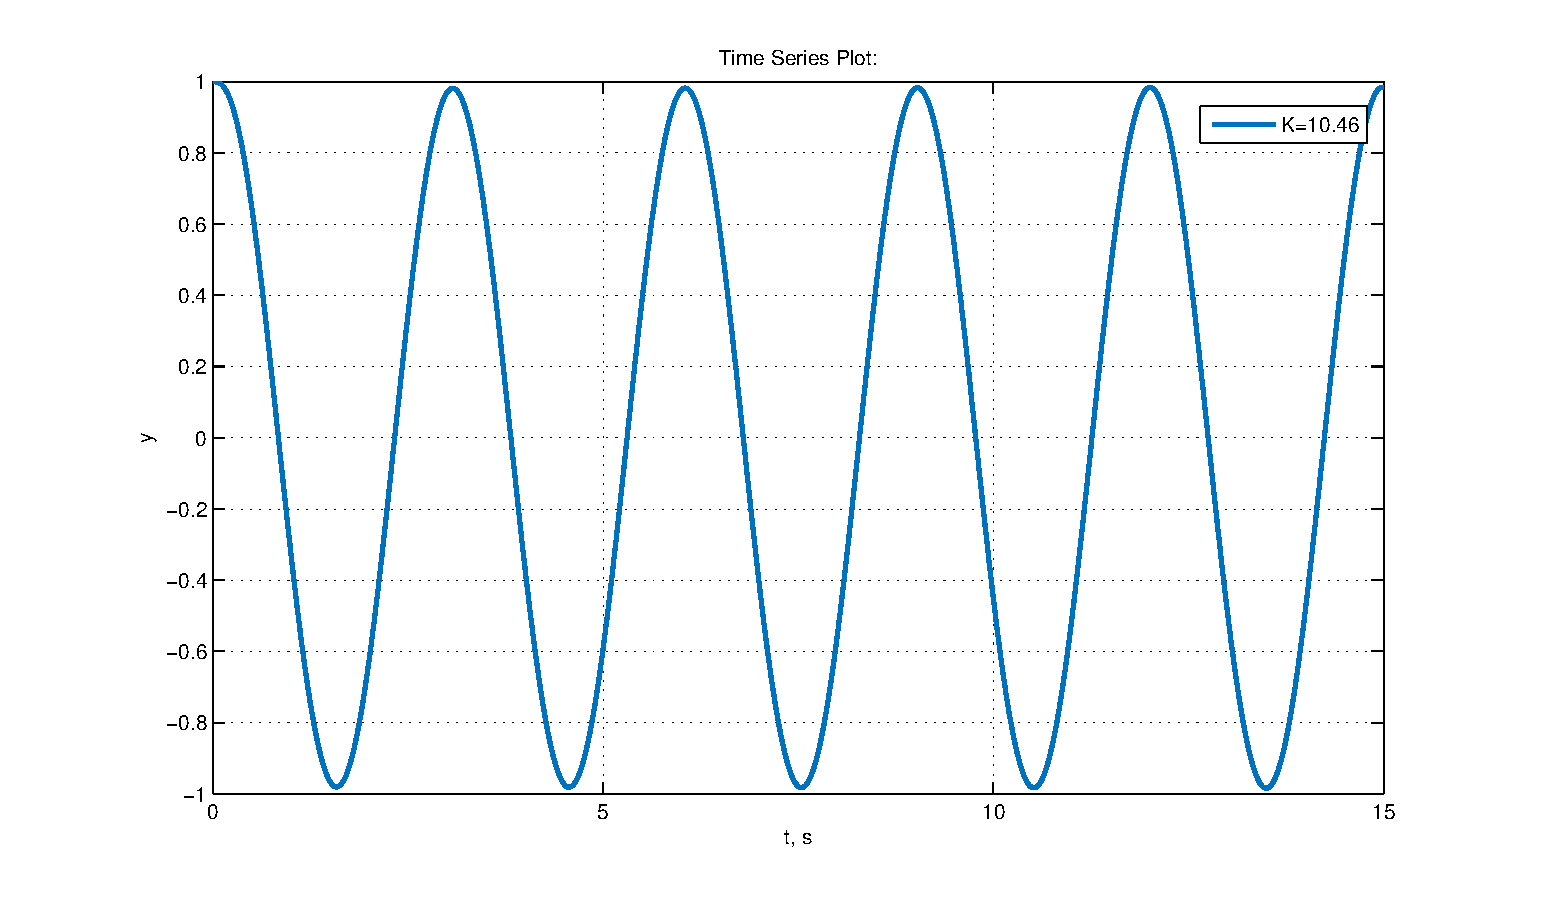
\includegraphics[width=1\linewidth]{first.eps}
	\caption{Система, находящаяся на границе устойчивости}
\end{figure}

\newpage
\begin{center}
    \section{Теоретический расчет границы устойчивости с использованием критерия Гурвица}
\end{center}
 
 
Передаточная функция замкнутой системы выглядит следующим образом:
\begin{equation} W(s) = \frac{\Phi(s)}{1 + \Phi(s)}, \end{equation}
где $\Phi(s)$ - передаточная функция разомкнутой системы.
\begin{equation} 
\Phi(s) = K\cdot\frac{1}{T_1s + 1}\cdot\frac{1}{T_2s + 1}\cdot\frac{1}{s} = \frac{K}{T_1T_2s^3 + (T_1 + T_2)s^2 +s},
\end{equation}
\par
Тогда \begin{equation} W(s) = \frac{K}{T_1T_2s^3 + (T_1 + T_2)s^2 +s + K}. \end{equation}
\par
На основании характеристического уравнения, построенного по передаточной функции замкнутой системы, составим матрицу Гурвица для определения границы устойчивости:
\[
\begin{vmatrix}
$$T_1 + T_2$$ & $$K$$ & 0\\
$$T_1T_2$$ & 1 & 0\\
0 & $$T_1 + T_2$$ & $$K$$
\end{vmatrix}
\]
\parПо критерию Гурвица для устойчивости системы необходимо, чтобы главные миноры матрицы были положительны. 
\begin{equation}
    \begin{cases}
        $$T_1 + T_2 > 0$$\\
        $$T_1 + T_2 - KT_1T_2 > 0$$\\
        $$K(T_1 + T_2) - K^2T_1T_2 > 0$$
    \end{cases}
\end{equation}
\parЕсли минор $n - 1$ порядка равен 0, то система будет находится на колебательной границе устойчивости. По условию $T_1$ и $T_2$ больше 0, тогда для определения границы устойчивости воспользуемся выражением:
\begin{equation}
    K = \frac{T_1 + T_2}{T_1T_2} =  \frac{1}{T_1} + \frac{1}{T_2}
\end{equation}
    
Используя выражение (5), найдём $K$. Полученные значения запишем в таблицу 2.
\begin{table}[h!]
	\caption{Данные, необходимые для построения теоретической границы устойчивости системы}
	\renewcommand{\arraystretch}{1.8} %строки
	\begin{tabular}{|c|c|c|c|c|c|c|c|c|c|c|}
		\hline $T_2$ & 0,1 & 0,5 & 1 & 1,5 & 2 & 2,5 & 3 & 3,5 & 4 & 5 \\
		\hline $K$ & 10,46 & 2,46 & 1,44 & 1,1 & 0,94 & 0,84 & 0,79 & 0,74 & 0,69 & 0,64 \\
		\hline
	\end{tabular}	
\end{table}  
 
По данным из таблицы 2 построим графическое изображение теоретической границы устойчивости (рисунок 5):
\begin{figure}[H]
	\centering
	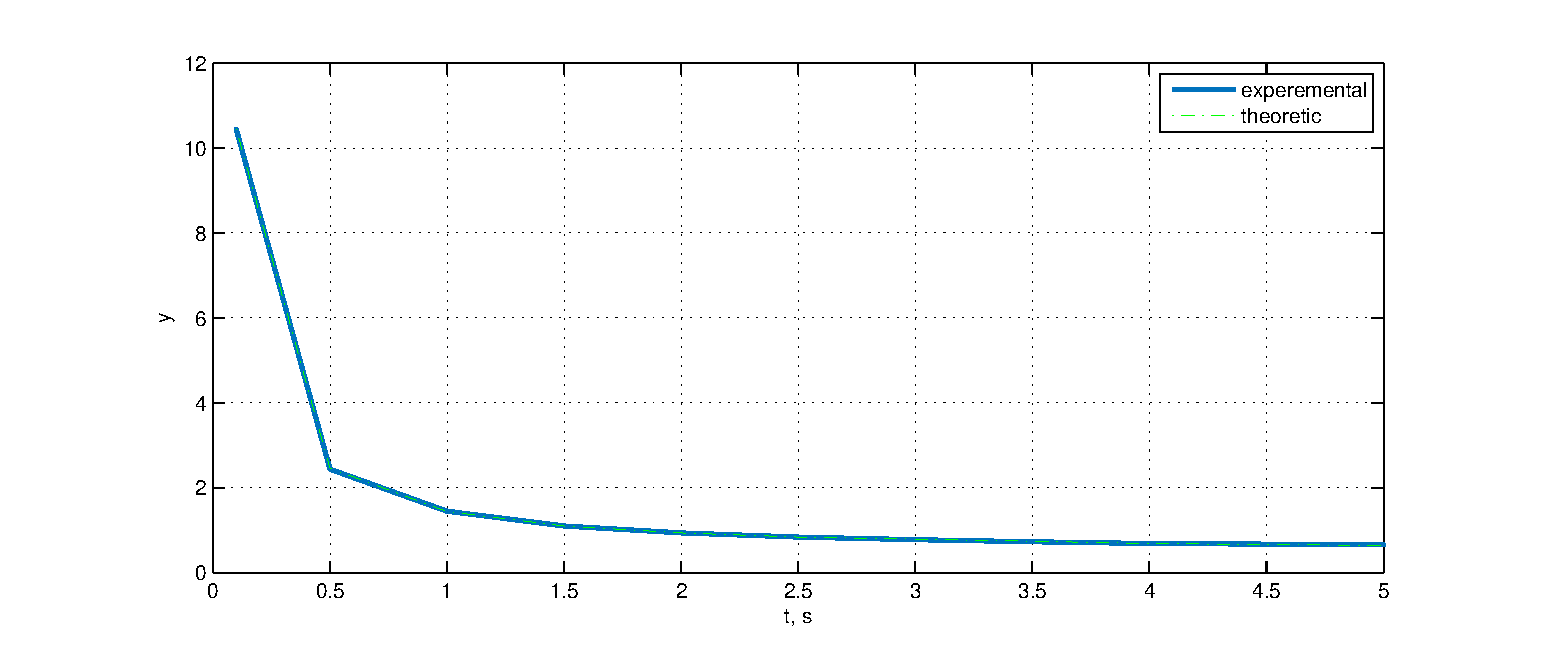
\includegraphics[width=1\linewidth]{forth.eps}
	\caption{Теоретическая и практическая границы устойчивости}
\end{figure}

\newpage
\section*{Вывод}
В ходе лабораторной работы был рассмотрен метод управления устойчивостью системы путём изменения отдельных её параметров, таких как  $T_2$ и $K$.
На основе критерия Гурвица были получены значения для построения графика границы устойчивости аналитическим методом. Аналитически полученные результаты приблизительно совпадают с полученными в результате математического моделирования.
Следовательно, устойчивость системы определяется не характером возмущения, а структурой самой системы.

\end{document}